\chapter{\bevezetes}

\section{A projekt célja}
A dokumentumban szereplő projekt célja snooker billiárdjáték felismerése, és analizálása fénykép/képernyőfelvétel alapján. A felismerés az asztalon elhelyezkedő különböző színű golyók pozíciójának meghatározásából áll. A felismerés megvalósításához különféle képfeldolgozási eszközöket, neurális hálózat alapú kép osztályozást használok, amelyeket \textbf{Python} programozási nyelven valósítok meg főként \textbf{OpenCV} és \textbf{Tensorflow} könyvtárak használatával. A bevezetés későbbi részeiben ismertetem a snooker billiárdjátékot, továbbá a projekt elkészítéséhez használt programozási nyelvet és fejlesztési könyvtárakat.

\section{A Snooker játék}
\subsection{Általánosságban a snooker játékról}
A snooker a billiárdjátékok egy bizonyos fajtája, amelyet egy zöld színű posztóval bevont asztalon játszanak, amelynek mérete általában 12 x 6 láb (365,8 cm x 182,9 cm)\cite{snooker_rules}. Az asztal négy sarkában és a két hosszabb oldal felénél ún. \textbf{zsebek} helyezkednek el. A játék célja a színes golyók belökése a fehér golyó segítségével a fent említett zsebekbe.

\subsection{Eszközök}
A játékot két fél játssza egymás ellen. A felek a lökéseiket egy hosszúkás, fából készült eszköz segítségével végzik. Ezt az eszközt \textbf{dákónak} nevezzük. A dákó vége, amellyel a golyó elütésre kerül, bőrrel van bevonva, amely a golyóval való kapcsolatot javítja. A dákón kívül a golyó elütéséhez a játékosok használhatnak segédeszközöket.
\par A tartozékok részei továbbá a már eddig is szóba került golyók. A játékhoz \textbf{22 db színes golyó} tartozik amelyek átmérője 52,5 mm.\cite{snooker_rules}
\newline Az egyes golyók különböző pontértékekkel rendelkeznek:\cite{snooker_rules}
\begin{itemize}
    \setlength\itemsep{-2pt}
    \item 1 db Fehér
    \item 15 db Piros - 1 pont
    \item 1 db Sárga - 2 pont
    \item 1 db Zöld - 3 pont
    \item 1 db Barna - 4 pont
    \item 1 db Kék - 5 pont
    \item 1 db Rózsaszín - 6 pont
    \item 1 db Fekete - 7 pont
\end{itemize}
A fehér golyó nem rendelkezik pontértékkel, mivel a játékosok ezt a golyót használják lökéseikhez.
\par A játék egy menetét \textbf{frémnek} nevezik, amely a kezdő lökéstől a fekete golyó elhelyezéséig tart.\cite{snooker_rules}
\begin{figure}[!ht]
    \centering
    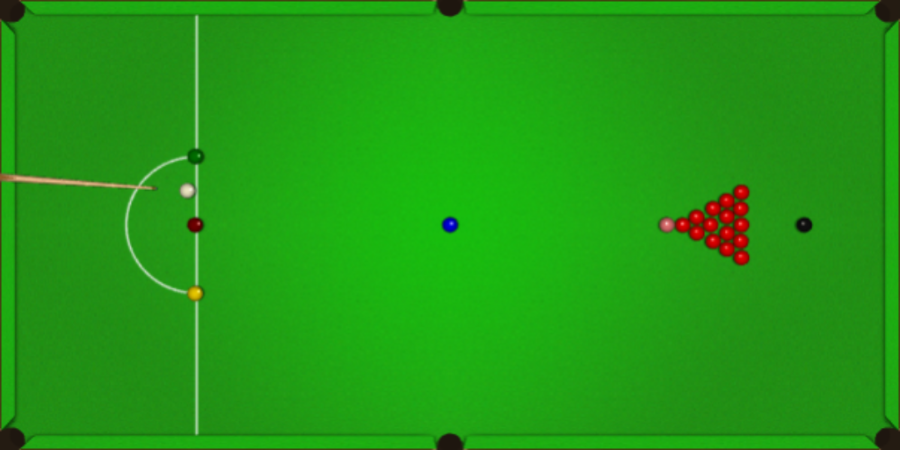
\includegraphics[width=100mm, keepaspectratio]{figures/starting_position.png}
    \caption{A golyók kezdeti pozíciója.}
    \label{fig:kezdeti_pozicio}
\end{figure}

\subsection{Pontszerzés}
A játékosok a pontjaikat a golyók bizonyos sorrendben való zsebbe helyezésével szerzik. Az egymás után hiba nélkül szerzett pontok összegét \textbf{törésnek} nevezzük. Egy játékos például szerzhet 9 pontos törést a következő golyók egymás utáni elhelyezésével \textit{piros -> zöld -> piros -> barna}.\cite{shamos2002new}
\par Egy játékos büntetőpontokat kap hibák elkövetése esetén. Hibát elkövetni lehet például a fehér golyó zsebbe helyezésével, nem megfelelő színű golyó elütésével. Az elkövetett hibáért minimum 4, maximum 7 pontlevonás jár, attól függően, hogy milyen színű golyók mozdulnak a hiba elkövetésekor (pl.: Ha a cél a piros golyó lelökése, de a lövő a feketét találja el, akkor 7 hibapont jár). A hibát elkövető játékos a törésének pontjait megkapja a hibát elkövetett lövés közben elhelyezett golyók pontjainak kivételével.\cite{snooker_rules}

\section{Az OpenCV képfeldolgozási könyvtár}
Az OpenCV egy főként \textbf{valós idejű képfeldolgozáshoz} használt programozási függvénykönyvtár. A könyvtár többféle programozási nyelvekhez készült implementációval létezik (pl.: C++, Python, Java stb.)\cite{opencv_2020}, ezek közül ebben a projektben Python programozási nyelven keresztül fogom használni.
\par A könyvtárból használt függvények segítségével kerülnek megnyitásra a képek, továbbá a képeken való műveletek (pl.: szürkeárnyalatolás, élkeresés) is a könyvtár segítségével lesznek végrehajtva. A későbbiekben lesz szó a könyvtárból használt függvényekről, azok működéséről nagyobb részletességben.

\section{Tensorflow a neurális hálózatokhoz}
A Tensorflow az OpenCV -hez hasonlóan egy függvénykönyvtár, azzal a különbséggel, hogy a könyvtár a \textbf{neurális hálózatok elkészítését és betanítását} teszi lehetővé.\cite{tensorflow} A neurális hálózatok közül itt főként neurális hálózatokat (Neural Network) fogok használni, amelyek a képfeldolgozás, kép osztályozás területén teljesítenek kiemelkedően. A könyvtár eszközeiről szintén részletesebben beszélek majd a későbbi fejezetekben.